% ==========================================================================
% INFO 4617 Web Data Science -- Week 16: Research Design & Final Presentations
%                                        (Chapter 15)
% Build:  TEXINPUTS=../common: BIBINPUTS=../common: latexmk -pdf slides.tex
% (or run `make` from the slides/ directory)
% ==========================================================================
\documentclass[9pt,aspectratio=169]{beamer}
% ==========================================================================
% Shared preamble for INFO 4617 Web Data Science weekly lecture decks
% Based on the Gotham beamer theme (vendored in this directory).
% Each week's slides.tex does:  % ==========================================================================
% Shared preamble for INFO 4617 Web Data Science weekly lecture decks
% Based on the Gotham beamer theme (vendored in this directory).
% Each week's slides.tex does:  % ==========================================================================
% Shared preamble for INFO 4617 Web Data Science weekly lecture decks
% Based on the Gotham beamer theme (vendored in this directory).
% Each week's slides.tex does:  \input{preamble}  (with common/ on TEXINPUTS)
% then sets \title/\subtitle/\author/\date and \begin{document}.
% ==========================================================================

\usetheme{gotham}

\usepackage{fbb}
\usepackage{booktabs}
\usepackage{graphicx}
\usepackage{tikz}
\usepackage{xcolor}
\usepackage{multirow}
\usepackage{listings}
\usetikzlibrary{positioning, arrows.meta, shapes}

% Bibliography
\usepackage[style=authoryear,
            backend=biber,
            maxcitenames=1,
            uniquename=false,
            uniquelist=false]{biblatex}
\addbibresource{bibliography.bib}

\gothamset{sectiontocframe default=off}

% ------------------------------------------------------------------ colors
\definecolor{cugold}{HTML}{CFB87C}
\definecolor{tab-red}{HTML}{E15759}
\definecolor{tab-orange}{HTML}{F28E2B}
\definecolor{tab-blue}{HTML}{4E79A7}
\definecolor{tab-cyan}{HTML}{76B7B2}
\definecolor{tab-green}{HTML}{59A14F}
\definecolor{tab-yellow}{HTML}{EDC948}
\definecolor{tab-purple}{HTML}{B07AA1}
\definecolor{tab-pink}{HTML}{FF9DA7}
\definecolor{tab-brown}{HTML}{9C755F}
\definecolor{tab-gray}{HTML}{BAB0AC}

\setbeamercolor{frametitle}{fg=black, bg=cugold}
\setbeamercolor{progress bar}{fg=cugold, bg=cugold!20}

\setbeamercolor{block title alerted}{fg=black, bg=cugold}
\setbeamercolor{block body alerted}{fg=black, bg=cugold!10}

% ------------------------------------------------------------------ footline
\setbeamertemplate{footline}{
  \begin{beamercolorbox}[wd=\paperwidth,ht=2.5ex,dp=1ex,right]{footline}
    {\footnotesize \insertframenumber{} of \inserttotalframenumber}
    \hspace*{2ex}
  \end{beamercolorbox}
}

% ------------------------------------------------------------------ helpers
\newcommand{\bottomcite}[1]{
    \vspace*{\fill}
    \vspace{-\baselineskip}
    {\tiny
    \rule{\textwidth}{0.3pt}\\
    #1
    }
    \vspace{0.5ex}
}

% Consistent code styling for the Wednesday "applied notebook" frames.
\lstdefinestyle{wds}{
    basicstyle=\ttfamily\scriptsize,
    keywordstyle=\color{tab-blue}\bfseries,
    commentstyle=\color{tab-green},
    stringstyle=\color{tab-orange},
    showstringspaces=false,
    breaklines=true,
    columns=fullflexible,
    language=Python,
    aboveskip=0.4em,
    belowskip=0.4em,
}
\lstset{style=wds}

% \dayband{Day}{Topic} -- a lightweight section divider label used to mark
% Monday / Wednesday / Friday within a week's deck.
\newcommand{\dayband}[2]{{\large\textbf{#1}}\;\textcolor{tab-gray}{\textbar}\;#2}
  (with common/ on TEXINPUTS)
% then sets \title/\subtitle/\author/\date and \begin{document}.
% ==========================================================================

\usetheme{gotham}

\usepackage{fbb}
\usepackage{booktabs}
\usepackage{graphicx}
\usepackage{tikz}
\usepackage{xcolor}
\usepackage{multirow}
\usepackage{listings}
\usetikzlibrary{positioning, arrows.meta, shapes}

% Bibliography
\usepackage[style=authoryear,
            backend=biber,
            maxcitenames=1,
            uniquename=false,
            uniquelist=false]{biblatex}
\addbibresource{bibliography.bib}

\gothamset{sectiontocframe default=off}

% ------------------------------------------------------------------ colors
\definecolor{cugold}{HTML}{CFB87C}
\definecolor{tab-red}{HTML}{E15759}
\definecolor{tab-orange}{HTML}{F28E2B}
\definecolor{tab-blue}{HTML}{4E79A7}
\definecolor{tab-cyan}{HTML}{76B7B2}
\definecolor{tab-green}{HTML}{59A14F}
\definecolor{tab-yellow}{HTML}{EDC948}
\definecolor{tab-purple}{HTML}{B07AA1}
\definecolor{tab-pink}{HTML}{FF9DA7}
\definecolor{tab-brown}{HTML}{9C755F}
\definecolor{tab-gray}{HTML}{BAB0AC}

\setbeamercolor{frametitle}{fg=black, bg=cugold}
\setbeamercolor{progress bar}{fg=cugold, bg=cugold!20}

\setbeamercolor{block title alerted}{fg=black, bg=cugold}
\setbeamercolor{block body alerted}{fg=black, bg=cugold!10}

% ------------------------------------------------------------------ footline
\setbeamertemplate{footline}{
  \begin{beamercolorbox}[wd=\paperwidth,ht=2.5ex,dp=1ex,right]{footline}
    {\footnotesize \insertframenumber{} of \inserttotalframenumber}
    \hspace*{2ex}
  \end{beamercolorbox}
}

% ------------------------------------------------------------------ helpers
\newcommand{\bottomcite}[1]{
    \vspace*{\fill}
    \vspace{-\baselineskip}
    {\tiny
    \rule{\textwidth}{0.3pt}\\
    #1
    }
    \vspace{0.5ex}
}

% Consistent code styling for the Wednesday "applied notebook" frames.
\lstdefinestyle{wds}{
    basicstyle=\ttfamily\scriptsize,
    keywordstyle=\color{tab-blue}\bfseries,
    commentstyle=\color{tab-green},
    stringstyle=\color{tab-orange},
    showstringspaces=false,
    breaklines=true,
    columns=fullflexible,
    language=Python,
    aboveskip=0.4em,
    belowskip=0.4em,
}
\lstset{style=wds}

% \dayband{Day}{Topic} -- a lightweight section divider label used to mark
% Monday / Wednesday / Friday within a week's deck.
\newcommand{\dayband}[2]{{\large\textbf{#1}}\;\textcolor{tab-gray}{\textbar}\;#2}
  (with common/ on TEXINPUTS)
% then sets \title/\subtitle/\author/\date and \begin{document}.
% ==========================================================================

\usetheme{gotham}

\usepackage{fbb}
\usepackage{booktabs}
\usepackage{graphicx}
\usepackage{tikz}
\usepackage{xcolor}
\usepackage{multirow}
\usepackage{listings}
\usetikzlibrary{positioning, arrows.meta, shapes}

% Bibliography
\usepackage[style=authoryear,
            backend=biber,
            maxcitenames=1,
            uniquename=false,
            uniquelist=false]{biblatex}
\addbibresource{bibliography.bib}

\gothamset{sectiontocframe default=off}

% ------------------------------------------------------------------ colors
\definecolor{cugold}{HTML}{CFB87C}
\definecolor{tab-red}{HTML}{E15759}
\definecolor{tab-orange}{HTML}{F28E2B}
\definecolor{tab-blue}{HTML}{4E79A7}
\definecolor{tab-cyan}{HTML}{76B7B2}
\definecolor{tab-green}{HTML}{59A14F}
\definecolor{tab-yellow}{HTML}{EDC948}
\definecolor{tab-purple}{HTML}{B07AA1}
\definecolor{tab-pink}{HTML}{FF9DA7}
\definecolor{tab-brown}{HTML}{9C755F}
\definecolor{tab-gray}{HTML}{BAB0AC}

\setbeamercolor{frametitle}{fg=black, bg=cugold}
\setbeamercolor{progress bar}{fg=cugold, bg=cugold!20}

\setbeamercolor{block title alerted}{fg=black, bg=cugold}
\setbeamercolor{block body alerted}{fg=black, bg=cugold!10}

% ------------------------------------------------------------------ footline
\setbeamertemplate{footline}{
  \begin{beamercolorbox}[wd=\paperwidth,ht=2.5ex,dp=1ex,right]{footline}
    {\footnotesize \insertframenumber{} of \inserttotalframenumber}
    \hspace*{2ex}
  \end{beamercolorbox}
}

% ------------------------------------------------------------------ helpers
\newcommand{\bottomcite}[1]{
    \vspace*{\fill}
    \vspace{-\baselineskip}
    {\tiny
    \rule{\textwidth}{0.3pt}\\
    #1
    }
    \vspace{0.5ex}
}

% Consistent code styling for the Wednesday "applied notebook" frames.
\lstdefinestyle{wds}{
    basicstyle=\ttfamily\scriptsize,
    keywordstyle=\color{tab-blue}\bfseries,
    commentstyle=\color{tab-green},
    stringstyle=\color{tab-orange},
    showstringspaces=false,
    breaklines=true,
    columns=fullflexible,
    language=Python,
    aboveskip=0.4em,
    belowskip=0.4em,
}
\lstset{style=wds}

% \dayband{Day}{Topic} -- a lightweight section divider label used to mark
% Monday / Wednesday / Friday within a week's deck.
\newcommand{\dayband}[2]{{\large\textbf{#1}}\;\textcolor{tab-gray}{\textbar}\;#2}


\title[Week 16 · Research Design]{{\Huge Research Design \& Final Presentations}}
\subtitle{Week 16 · Practice module · Textbook Chapter 15}
\author[Keegan]{\textbf{Brian C. Keegan, Ph.D.} \\ Associate Professor, Department of Information Science \\ University of Colorado Boulder}
\date{November 30, December 2 \& 4, 2026}

\begin{document}

\maketitle

% -------------------------------------------------------------------------
\begin{frame}{This week at a glance}
    \begin{columns}[T]
        \begin{column}{0.62\textwidth}
            We close the course by turning \textbf{technique into knowledge}: how to design a research project around web data --- and then present your own.

            \vspace{1em}

            \dayband{Monday}{Concepts}
            \begin{itemize}\small
                \item From question to data source; matching designs; sampling, bias \& validity
            \end{itemize}

            \vspace{0.5em}

            \dayband{Wednesday}{Project workshop}
            \begin{itemize}\small
                \item Match \textit{your} source to a design, scope feasibility, and trade peer feedback --- no new code
            \end{itemize}

            \vspace{0.5em}

            \dayband{Friday}{Final presentations}
            \begin{itemize}\small
                \item Present your project --- the last day of class
            \end{itemize}
        \end{column}
        \begin{column}{0.34\textwidth}
            \begin{block}{Companion notebook}
                \footnotesize \texttt{ch-15-research-design.ipynb}
            \end{block}
            \begin{alertblock}{Last week of the course}
                \footnotesize Friday (Dec.~4) is the final class --- campus runs a Monday schedule. The \textbf{project repo \& write-up are due Fri.\ Dec.~11}.
            \end{alertblock}
        \end{column}
    \end{columns}
\end{frame}

% =========================================================================
\section{Monday · Concepts}
% =========================================================================

\begin{frame}{Technical skill is not enough}
    \begin{columns}[T]
        \begin{column}{0.58\textwidth}
            You now command the whole toolkit: scrape static (Ch.~6) and dynamic (Ch.~8) pages, parse PDFs (Ch.~9), query APIs from Wikipedia to Spotify to the Fed (Ch.~10--12), apply NLP and LLMs (Ch.~13), and automate collection (Ch.~14).

            \vspace{0.8em}

            But \textbf{technical skill without research design produces data, not knowledge.} A flawless scraper pointed at the wrong question still answers nothing.

            \vspace{0.8em}

            This week steps back from code to the questions that decide whether excellent scraping yields real insight.
        \end{column}
        \begin{column}{0.38\textwidth}
            \begin{alertblock}{Four questions design must answer}
                \footnotesize
                \begin{itemize}\footnotesize
                    \item What is the \textbf{right question} for this source?
                    \item What can this data \textbf{actually} tell you?
                    \item What are the \textbf{threats to validity}?
                    \item How do you \textbf{communicate} findings responsibly?
                \end{itemize}
            \end{alertblock}
        \end{column}
    \end{columns}
    \bottomcite{Textbook Ch.~15, ``Technical Skill Is Not Enough.'' The tools are means; knowledge is the end.}
\end{frame}

\begin{frame}{From question to data source: the proposal arc}
    \begin{columns}[T]
        \begin{column}{0.56\textwidth}
            The best projects start with a \textbf{question, not a dataset} --- the source serves the question. Every proposal (class project, thesis, paper, grant) shares one arc:
            \begin{enumerate}\small
                \item \textbf{Motivation} --- what problem, why it matters, who benefits
                \item \textbf{Data source} --- which web data, what constructs, what gaps
                \item \textbf{Methods} --- how you collect \& analyze it
                \item \textbf{Expected results} --- what analyses \& figures
                \item \textbf{Implications} --- what stakeholders should do
                \item \textbf{Limitations} --- what the data \textit{cannot} tell you
            \end{enumerate}

            \vspace{0.5em}

            \textbf{Limitations are not an afterthought} --- naming what your data cannot do is as important as showing what it can.
        \end{column}
        \begin{column}{0.4\textwidth}
            \centering
            
\includegraphics[width=\textwidth]{img/proposal_arc.png}\\
            {\scriptsize The same arc structures a proposal, a write-up, and a talk.}
        \end{column}
    \end{columns}
    \bottomcite{Textbook Ch.~15, ``The Proposal Arc.''}
\end{frame}

\begin{frame}{Matching questions to designs}
    Your question implies a design; the design implies which chapters' tools you reach for:
    \begin{center}\small
    \begin{tabular}{@{}p{0.24\textwidth}p{0.34\textwidth}p{0.34\textwidth}@{}}
        \toprule
        \textbf{Design} & \textbf{Web data methods} & \textbf{Example question} \\
        \midrule
        Longitudinal tracking & Wayback Machine (Ch.~7), Actions (Ch.~14) & How has a privacy policy changed over time? \\
        Cross-sectional snapshot & API queries (Ch.~10--12) & How does Reddit moderation differ across subreddits? \\
        Content analysis & Scraping (Ch.~6) + LLM coding (Ch.~13) & What topics dominate Colorado legislation? \\
        Network analysis & Link \& social-graph extraction (Ch.~10, 12) & How connected are climate articles on Wikipedia? \\
        Natural experiment & Event-triggered collection (Ch.~14) & How did a policy change shift search patterns? \\
        \bottomrule
    \end{tabular}
    \end{center}
    \vspace{0.4em}
    {\footnotesize \textbf{Design considerations vary.} Longitudinal: Wayback snapshots are uneven; scrapers need upkeep. Cross-sectional: \textbf{selection bias} --- you get only platforms that exist and expose the variable. Content analysis: validate automated coding against a hand-coded sample. Natural experiment: causal claims are always tentative --- you need a clear treatment and a defensible comparison group.}
    \bottomcite{Textbook Ch.~15, ``Matching Questions to Methods'' \& ``Common Research Designs with Web Data.''}
\end{frame}

\begin{frame}{Web data is not a random sample}
    \begin{columns}[T]
        \begin{column}{0.56\textwidth}
            Every design inherits one problem: web data is a \textbf{convenience sample}, shaped by who uses the platform, what the API exposes, and what your scraper can reach.
            \begin{itemize}\small
                \item \textbf{Who is missing?} Reddit skews young, male, American; Wikipedia editors skew educated \& Global North.
                \item \textbf{What is hidden?} APIs expose what platforms \textit{choose} to --- not deleted posts, shadow-bans, or ranking algorithms.
                \item \textbf{What is lost?} Pages are deleted and redesigned; yesterday's data may already be gone (Ch.~3).
            \end{itemize}

            \vspace{0.4em}

            \textbf{Construct validity}: does the thing you can measure (pageviews, posts, queries) match the concept you claim to study (attention, opinion, illness)? Weak construct validity is the most common flaw.
        \end{column}
        \begin{column}{0.4\textwidth}
            \centering
            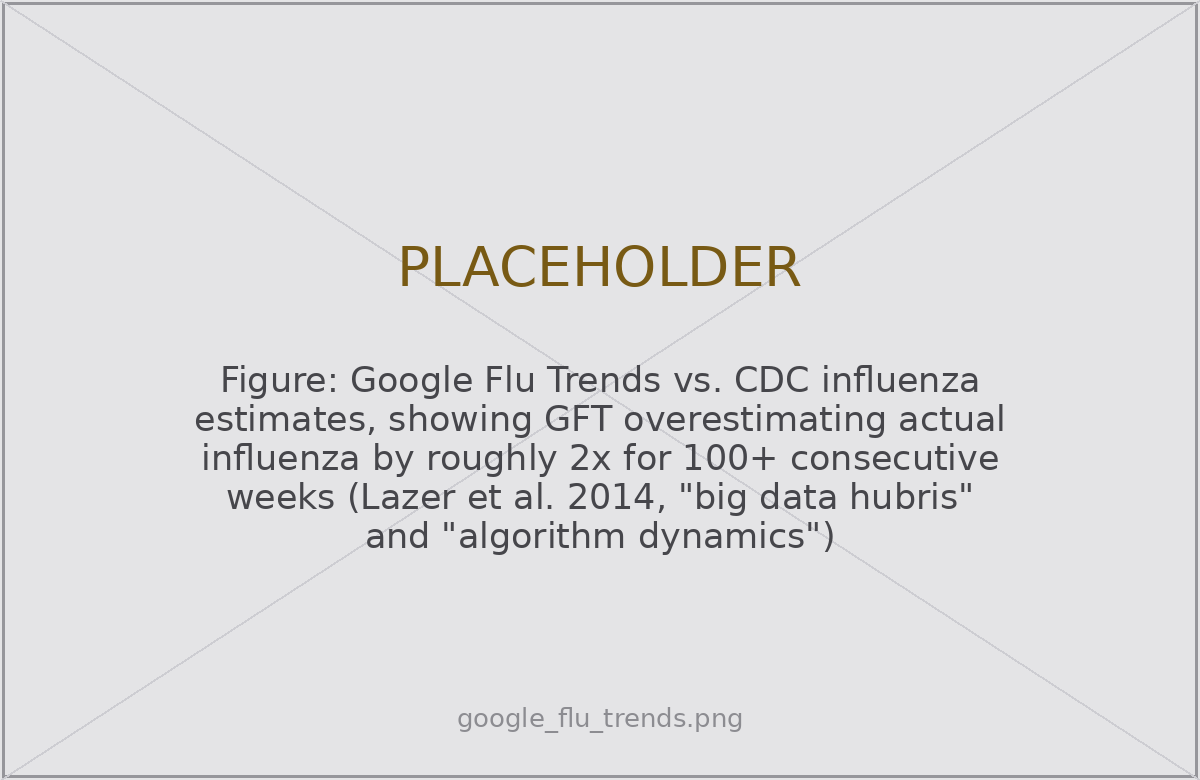
\includegraphics[width=\textwidth]{img/google_flu_trends.png}\\
            {\scriptsize Google Flu Trends overestimated flu $\sim$2$\times$ for 100+ weeks: \textit{big-data hubris} plus \textit{algorithm dynamics} --- the instrument drifted while the phenomenon held still.}
        \end{column}
    \end{columns}
    \bottomcite{Textbook Ch.~15, ``Sampling and Representativeness.'' Construct validity: \textcite{salganik2018bit}; the cautionary tale: \textcite{lazer2014parable}.}
\end{frame}

\begin{frame}{Human subjects \& the IRB}
    \begin{columns}[T]
        \begin{column}{0.58\textwidth}
            If your data is about \textbf{people} --- and most web data is --- you may be doing \textbf{human subjects research}. That is not a call you make for yourself.
            \begin{itemize}\small
                \item \textbf{Public does not mean exempt.} ``It was on the public web'' is about access, not ethics. The \textbf{IRB} makes the determination --- if you think ``obviously fine, I won't ask,'' that is exactly when to ask.
                \item \textbf{Terms of service are not an ethics review} (Ch.~2) --- a legal matter, separate from the human-subjects question.
                \item \textbf{Minimize \& de-identify by default} --- collect only the fields you need; hash or drop the rest.
            \end{itemize}
        \end{column}
        \begin{column}{0.4\textwidth}
            \begin{block}{Consult early when you\dots}
                \footnotesize
                \begin{itemize}\footnotesize
                    \item interact with users (even a message)
                    \item collect from private / invite-only spaces
                    \item identify specific individuals
                    \item measure sensitive attributes (health, sexuality, immigration, politics)
                \end{itemize}
            \end{block}
            {\footnotesize \textbf{This class:} your instructor is the checkpoint. \textbf{Publishing (5617):} request an IRB determination early.}
        \end{column}
    \end{columns}
    \bottomcite{Textbook Ch.~15, ``Human Subjects and the IRB.'' See \textcite{fiesler2020no} and the ethics appendix of \textcite{salganik2018bit}.}
\end{frame}

% =========================================================================
\section{Wednesday · Project Workshop}
% =========================================================================

\begin{frame}{Wednesday: design your own project}
    \begin{columns}[T]
        \begin{column}{0.6\textwidth}
            Today is a \textbf{workshop}, not a notebook. You proposed a project back in Week~10 --- now we harden it into something you can execute, defend, and present.

            \vspace{0.8em}

            Three activities, in pairs:
            \begin{enumerate}\small
                \item \textbf{Draft} --- write your project against the six-part proposal arc.
                \item \textbf{Scope} --- match your source to a design and stress-test its feasibility.
                \item \textbf{Review} --- trade drafts and give kind, specific, actionable feedback.
            \end{enumerate}

            \vspace{0.6em}

            Bring what you have: a question, a candidate data source, and any data you have already pulled this semester.
        \end{column}
        \begin{column}{0.36\textwidth}
            \begin{alertblock}{The goal}
                \footnotesize Leave today with a design you could \textbf{write down in full} --- because a design you cannot write down is a design you have not finished.
            \end{alertblock}
        \end{column}
    \end{columns}
    \bottomcite{Textbook Ch.~15, ``Managing the Research Process.'' Feedback ethos reused from the Friday revision workflow.}
\end{frame}

\begin{frame}{Activity 1 --- draft your six-part design}
    \begin{columns}[T]
        \begin{column}{0.56\textwidth}
            Fill in one crisp sentence for each. Vague answers now become dead ends later:
            \begin{enumerate}\small
                \item \textbf{Motivation} --- ``I want to know \underline{\hspace{5em}} because \underline{\hspace{4em}}.''
                \item \textbf{Data source} --- name the site/API and the \textbf{construct} each field measures.
                \item \textbf{Methods} --- which chapters' tools, and in what order.
                \item \textbf{Expected results} --- the actual figure or table you picture.
                \item \textbf{Implications} --- who acts on the answer, and how.
                \item \textbf{Limitations} --- the honest ``this cannot tell you\dots''.
            \end{enumerate}
        \end{column}
        \begin{column}{0.4\textwidth}
            \centering
            
\includegraphics[width=\textwidth]{img/design_canvas.png}\\
            {\scriptsize One page, six boxes --- if a box is blank, that is where the project is weakest.}
        \end{column}
    \end{columns}
    \bottomcite{Textbook Ch.~15, ``The Proposal Arc.'' Exercise 1: a 1{,}500-word version of exactly this.}
\end{frame}

\begin{frame}{Activity 2 --- scope feasibility}
    \begin{columns}[T]
        \begin{column}{0.5\textwidth}
            First, \textbf{name your unit of analysis} --- is a row a post, a user, a day, or a community? Deciding after collection means collecting again.

            \vspace{0.6em}

            Then run the \textbf{pitfalls checklist} against your design:
            \begin{itemize}\small
                \item Am I \textbf{sampling on the outcome}? (only viral posts $\Rightarrow$ can't explain virality)
                \item Bot \& spam \textbf{contamination} filtered?
                \item \textbf{Survivorship} --- what deleted/suspended content is invisible?
                \item Will I \textbf{change instrumentation} mid-collection? (self-inflicted drift)
            \end{itemize}
        \end{column}
        \begin{column}{0.46\textwidth}
            \begin{block}{Can you actually collect it?}
                \footnotesize
                \begin{itemize}\footnotesize
                    \item Rate limits \& volume --- does it finish in time?
                    \item ToS \& \texttt{robots.txt} clear? (Ch.~2)
                    \item IRB checkpoint needed?
                    \item Erosion risk --- capture \textbf{now} or lose it? (Ch.~3)
                \end{itemize}
            \end{block}
            \begin{alertblock}{Validate early}
                \footnotesize Wire a \texttt{validate\_dataset()} check into collection \textit{now}, not at analysis --- or you discover a June redesign emptied half your columns in September.
            \end{alertblock}
        \end{column}
    \end{columns}
    \bottomcite{Textbook Ch.~15, ``Common Pitfalls'' \& ``Data Quality and Validation.''}
\end{frame}

\begin{frame}{Activity 3 --- peer review}
    \begin{columns}[T]
        \begin{column}{0.6\textwidth}
            Swap designs with your partner. Read it as a friendly skeptic and answer four questions in writing:
            \begin{enumerate}\small
                \item Is the \textbf{question actually answerable} with this source?
                \item What is the \textbf{single biggest threat to validity}?
                \item What is \textbf{missing, hidden, or lost} in this sample?
                \item One \textbf{concrete} thing that would make it stronger.
            \end{enumerate}

            \vspace{0.6em}

            Same ethos as our Friday code reviews: \textbf{kind, specific, actionable} --- name the line and the claim, assume good faith, end with a clear verdict.
        \end{column}
        \begin{column}{0.36\textwidth}
            \begin{block}{Give feedback that helps}
                \footnotesize
                \begin{itemize}\footnotesize
                    \item Point to the \textit{design}, not the person
                    \item Separate ``must fix'' from ``nice to have''
                    \item Offer a fix, not just a flaw
                \end{itemize}
            \end{block}
            {\footnotesize You get the same in return --- take one reviewer's biggest concern and revise before Friday.}
        \end{column}
    \end{columns}
    \bottomcite{Textbook Ch.~15, ``Sampling and Representativeness'' as the review lens.}
\end{frame}

\begin{frame}[fragile]{Reproducible from day one}
    Your final deliverable is a \textbf{repository}, so structure it like one now --- someone else (or you in six months) should re-run it and get the same results:
    \begin{columns}[T]
        \begin{column}{0.52\textwidth}
\begin{lstlisting}[language=bash]
my-project/
  .gitignore        # keep keys & big data out
  README.md         # overview + setup
  requirements.txt  # PINNED versions
  data/
    raw/            # scraped data, NEVER edited
    processed/      # cleaned data
    README.md       # datasheet lives here
  notebooks/        # 01_collection ... 03_analysis
  scripts/          # scraper.py
  output/           # figures/ tables/
\end{lstlisting}
        \end{column}
        \begin{column}{0.44\textwidth}
            \begin{block}{Write a datasheet}
                \footnotesize For every dataset, record:
                \begin{itemize}\footnotesize
                    \item \textbf{What} each variable measures \& units
                    \item \textbf{How} --- tools, params, filters, date range
                    \item \textbf{Limits} --- what is not captured; likely biases
                    \item \textbf{Ethics} --- PII? ToS-compliant? safe to share?
                \end{itemize}
            \end{block}
            {\footnotesize Openness is a \textbf{design choice}: pinned environments and archived raw data stay verifiable even as platforms erode.}
        \end{column}
    \end{columns}
    \bottomcite{Textbook Ch.~15, ``Reproducibility'' \& ``Data Documentation.'' Datasheets: \textcite{gebru2021datasheets}. Git: \textit{Missing Manual} Ch.~31.}
\end{frame}

\begin{frame}[standout]
    A design you cannot write down\\
    is a design you have not finished.\\[1em]
    Specify the question, the source, the unit,\\
    and the limitation --- \textit{before} you collect.\\[1em]
    {\large The discipline of writing it down \textit{is} the method.}
\end{frame}

% =========================================================================
\section{Friday · Final Presentations}
% =========================================================================

\begin{frame}{Friday: final presentations}
    \begin{columns}[T]
        \begin{column}{0.6\textwidth}
            The last day of class --- you present the project you designed this week.

            \vspace{0.8em}

            \textbf{Logistics}
            \begin{itemize}\small
                \item $\sim$6 minutes per team + 2 minutes of questions
                \item Follow the \textbf{proposal arc}: motivation $\to$ data $\to$ methods $\to$ results $\to$ implications $\to$ limitations
                \item Slides or a live notebook --- your choice; \textbf{practice the timing}
                \item Everyone presents; everyone asks at least one question
            \end{itemize}
        \end{column}
        \begin{column}{0.36\textwidth}
            \begin{alertblock}{Two deadlines}
                \footnotesize
                \textbf{Today (Dec.~4)} --- present your work in class.\\[0.4em]
                \textbf{Fri.\ Dec.~11} --- the polished \textbf{project repository \& write-up} are due. Present now; harden the write-up with the week's feedback.
            \end{alertblock}
        \end{column}
    \end{columns}
    \bottomcite{Textbook Ch.~15, ``Communicating Findings.'' The talk is the proposal arc, spoken.}
\end{frame}

\begin{frame}{What a strong final presentation looks like}
    \begin{columns}[T]
        \begin{column}{0.5\textwidth}
            \begin{block}{Do}
                \footnotesize
                \begin{itemize}\footnotesize
                    \item Lead with the \textbf{``so what?''} --- the finding, not the plumbing
                    \item State a \textbf{claim}, then show the evidence for it
                    \item Be \textbf{honest about limitations} --- it reads as strength, not weakness
                    \item Know your \textbf{audience} \& its evidentiary bar
                    \item Show your work: methods reproducible from the description
                \end{itemize}
            \end{block}
        \end{column}
        \begin{column}{0.46\textwidth}
            \begin{block}{Same finding, three audiences}
                \footnotesize
                \begin{itemize}\footnotesize
                    \item \textbf{Academic} --- precision, explicit limits, prior work; replicable methods
                    \item \textbf{Policy brief} --- actionable, plain language; lead with implications
                    \item \textbf{Data journalism} --- narrative, visual evidence, accountability framing
                \end{itemize}
            \end{block}
            {\footnotesize Pick the register that fits \textit{your} question --- and commit to it.}
        \end{column}
    \end{columns}
    \bottomcite{Textbook Ch.~15, ``Communicating Findings.''}
\end{frame}

\begin{frame}{Your visualizations are arguments}
    \begin{columns}[T]
        \begin{column}{0.5\textwidth}
            A default \texttt{plt.plot()} makes the reader \textbf{guess}. A designed figure \textbf{argues}:
            \begin{itemize}\small
                \item Title states a \textbf{finding}, not the axes (``\dots spikes around legislative and health crises,'' not ``Pageviews over time'')
                \item \textbf{Annotate} peaks with the events that caused them
                \item Axis labels carry \textbf{units}
                \item Kill chart junk --- drop the top \& right spines
            \end{itemize}

            \vspace{0.4em}

            Test: if a reader saw \textit{only} this image and its title, would they get your claim?

            \vspace{0.5em}

            {\footnotesize \textbf{A model to steal from:} ProPublica's \textit{Dollars for Docs} --- question $\to$ scrape hidden disclosures $\to$ clean \& link $\to$ public database. Journalists publish code, describe cleaning, and state limits --- exactly our reproducibility standard.}
        \end{column}
        \begin{column}{0.46\textwidth}
            \centering
            
\includegraphics[width=\textwidth]{img/aca_pageviews_annotated.png}\\
            {\scriptsize The title makes the claim; the annotations supply the evidence.}
        \end{column}
    \end{columns}
    \bottomcite{Textbook Ch.~15, ``Visualization as Argument'' \& ``Data Journalism as a Model.''}
\end{frame}

\begin{frame}{The deliverable --- and the values behind it}
    \begin{columns}[T]
        \begin{column}{0.52\textwidth}
            \textbf{Due Friday, December 11} --- a repository plus a write-up:
            \begin{itemize}\small
                \item Reproducible repo: \texttt{README}, pinned \texttt{requirements.txt}, untouched \texttt{data/raw/}, a datasheet
                \item Write-up structured as the six-part arc, limitations included
                \item Figures that argue; methods replicable from the text
            \end{itemize}

            \vspace{0.5em}

            The tools you learned are \textbf{means, not ends}. The end is knowledge that serves three values from Ch.~3:
        \end{column}
        \begin{column}{0.44\textwidth}
            \begin{block}{Openness, Oversight, Ownership}
                \footnotesize
                \begin{itemize}\footnotesize
                    \item \textbf{Openness} --- publish code, data (where ethical), methods so others can build on it
                    \item \textbf{Oversight} --- does it help citizens \& journalists understand systems that affect them?
                    \item \textbf{Ownership} --- are you building reusable infrastructure, or extracting without contributing back?
                \end{itemize}
            \end{block}
        \end{column}
    \end{columns}
    \bottomcite{Textbook Ch.~15, ``Public Interest Connection'' \& ``Social History and Public Interest.'' Values from Ch.~3.}
\end{frame}

% =========================================================================
\begin{frame}{Key takeaways}
    \begin{enumerate}
        \item \textbf{Start with a question, not a dataset} --- the source serves the question, and the proposal arc runs motivation $\to$ limitations.
        \item \textbf{Match the design to the claim} --- longitudinal, cross-sectional, content analysis, network, or natural experiment, each with its own threats.
        \item \textbf{Web data is a convenience sample} --- ask who is missing, what is hidden, what is lost, and whether your variable has \textbf{construct validity}.
        \item \textbf{``Public'' is not ``exempt.''} Consult the IRB, minimize and de-identify, and document the dataset with a datasheet.
        \item \textbf{Communicate responsibly} --- reproducible pipelines, honest limitations, and figures that argue in service of openness, oversight, and ownership.
    \end{enumerate}
    \vspace{0.8em}
    \bottomcite{Reading: Textbook Ch.~15. Related: \textcite{salganik2018bit}; \textcite{gebru2021datasheets}; \textcite{lazer2020computational}; \textcite{vanatteveldt2022computational}; \textcite{rogers2019doing}.}
\end{frame}

\begin{frame}[standout]
    That is the course.\\[0.6em]
    You can reach almost any data on the web ---\\
    and you know when you \textit{should}, what it can mean,\\
    and how to tell someone honestly.\\[1em]
    {\large Go make the web legible. Thank you.}
\end{frame}

\end{document}
